\subsection{Python implementation}
The code has been developed in Python 3 and it is contained in classes. The main swapping function is callable as a method class within the ITI's main module. The inner loops are split in protected methods, since they are made to work internally. There’s a protected method for each level of depth in the loops of the algorithm described in \ref{section:methods:pipeline}.The information is shared among them via custom objects or the global class attributes.
\\

Aside the main objects, there is a Metadata object which stores all the information for future preprocessing of the data and allows recovery on the same spot the execution ended, either due to an intended halt or an error.
Data for preprocessing is highly important since we require results normalisation.

% \subsection{Edge Evolution on moving threshold}
% \label{suppl:relations}
% % Not-normalised
% \begin{figure}[!htb]
% 	\centering
% 	\begin{subfigure}[b]{0.15\linewidth}
% 		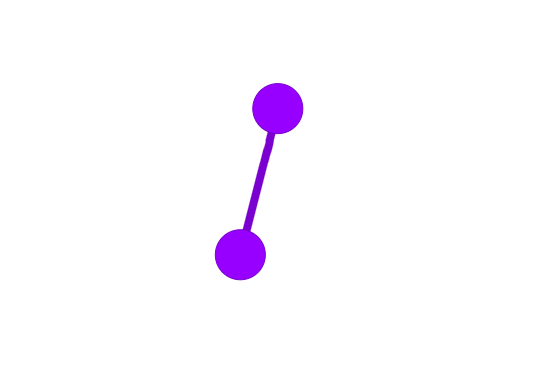
\includegraphics[width=\linewidth]{Minor Thesis/figures/graphs/nn/A.png}
% 		\caption{max(index)}
% 	\end{subfigure}
% 	\hfill
% 	\begin{subfigure}[b]{0.15\linewidth}
% 		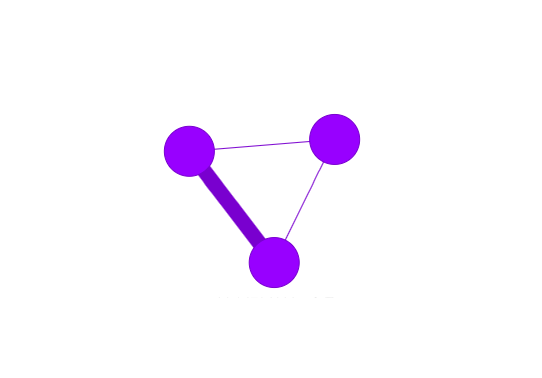
\includegraphics[width=\linewidth]{Minor Thesis/figures/graphs/nn/B.png}
% 		\caption{max(index)-1}
% 	\end{subfigure}
% 	\hfill
% 	\begin{subfigure}[b]{0.15\linewidth}
% 		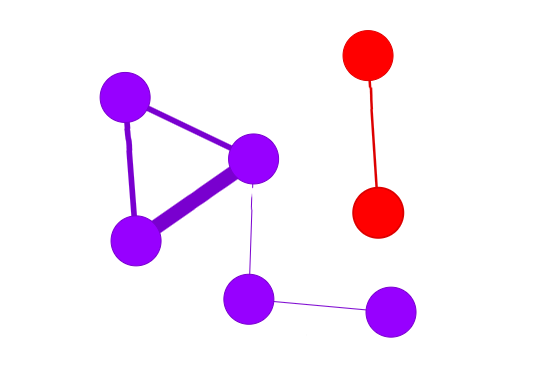
\includegraphics[width=\linewidth]{Minor Thesis/figures/graphs/nn/C.png}
% 		\caption{max(index)-2}
% 	\end{subfigure}
% 	\hfill
% 	\begin{subfigure}[b]{0.15\linewidth}
% 		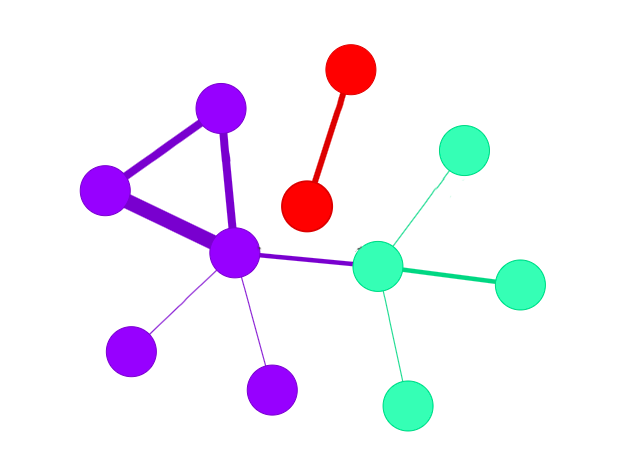
\includegraphics[width=\linewidth]{Minor Thesis/figures/graphs/nn/D.png}
% 		\caption{max(index)-3}
% 	\end{subfigure}
% 	\hfill
% 	\begin{subfigure}[b]{0.15\linewidth}
% 		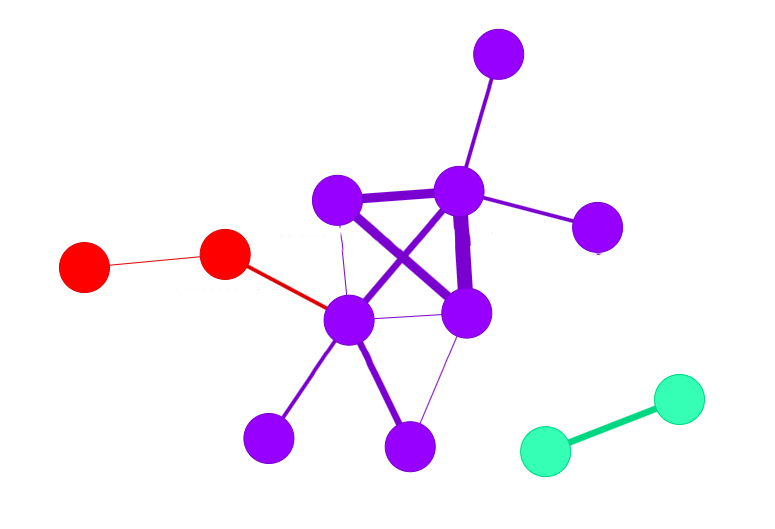
\includegraphics[width=\linewidth]{Minor Thesis/figures/graphs/nn/E.png}
% 		\caption{max(index)-4}
% 	\end{subfigure}
% 	\hfill
% 	\begin{subfigure}[b]{0.15\linewidth}
% 		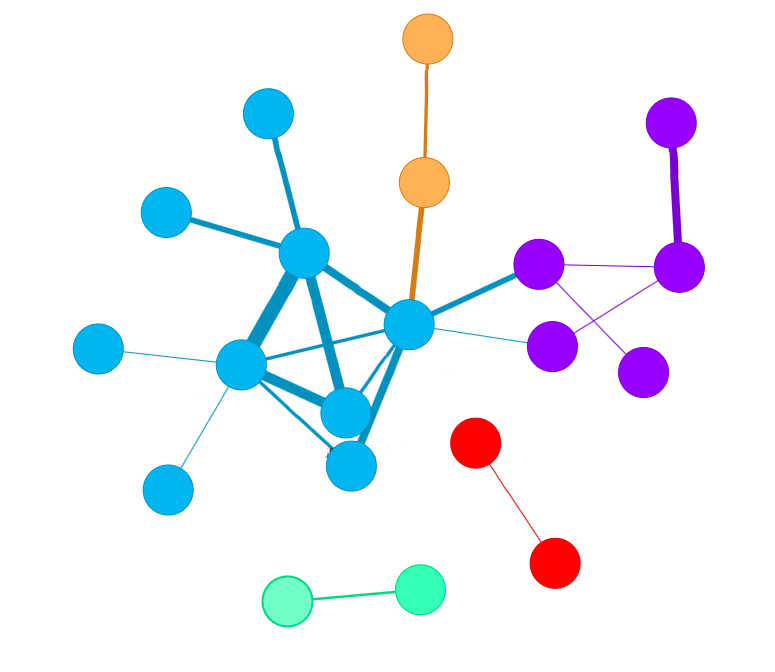
\includegraphics[width=\linewidth]{Minor Thesis/figures/graphs/nn/F.png}
% 		\caption{max(index)-5}
% 	\end{subfigure}
% 	\caption{Graph building evolution. Not-normalised results. We indicate values and position as: for (value, index) $\in$ Ascending Ordered Weights, i.e. the highest index contains the highest weight.}
% 	\label{fig:graph-evo-nn}
% \end{figure}

% % Normalised
% \begin{figure}[!htb]
% 	\centering
% 	\begin{subfigure}[b]{0.13\linewidth}
% 		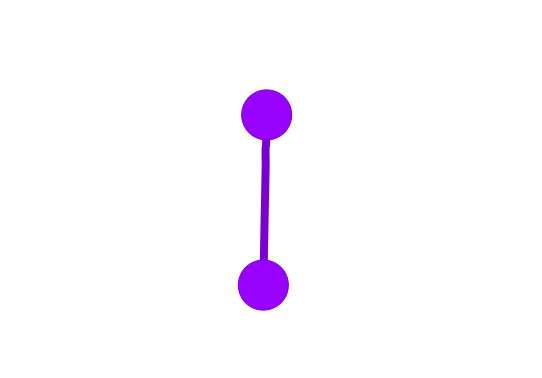
\includegraphics[width=\linewidth]{Minor Thesis/figures/graphs/sa/A.png}
% 		\caption{max(index)}
% 	\end{subfigure}
% 	\hfill
% 	\begin{subfigure}[b]{0.13\linewidth}
% 		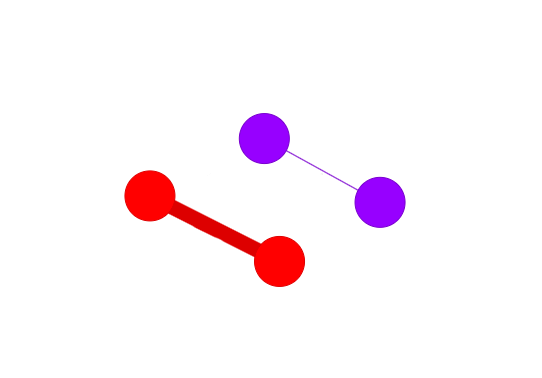
\includegraphics[width=\linewidth]{Minor Thesis/figures/graphs/sa/B.png}
% 		\caption{max(index)-1}
% 	\end{subfigure}
% 	\hfill
% 	\begin{subfigure}[b]{0.13\linewidth}
% 		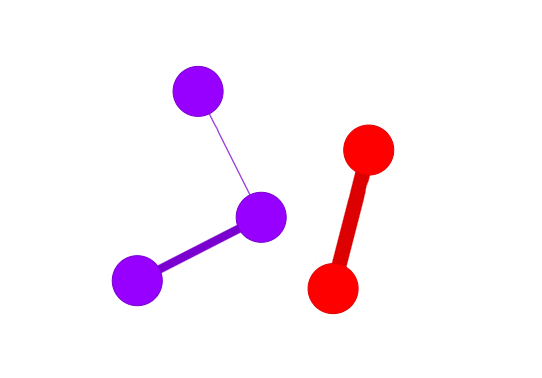
\includegraphics[width=\linewidth]{Minor Thesis/figures/graphs/sa/C.png}
% 		\caption{max(index)-2}
% 	\end{subfigure}
% 	\hfill
% 	\begin{subfigure}[b]{0.13\linewidth}
% 		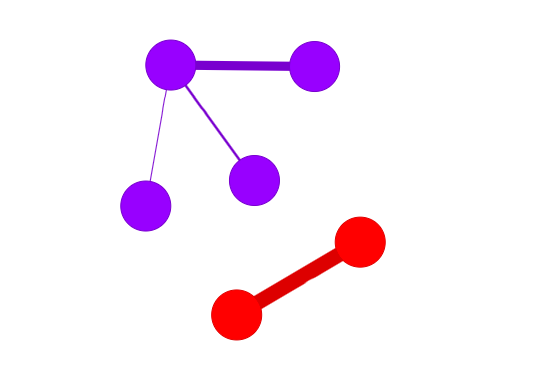
\includegraphics[width=\linewidth]{Minor Thesis/figures/graphs/sa/D.png}
% 		\caption{max(index)-3}
% 	\end{subfigure}
% 	\hfill
% 	\begin{subfigure}[b]{0.13\linewidth}
% 		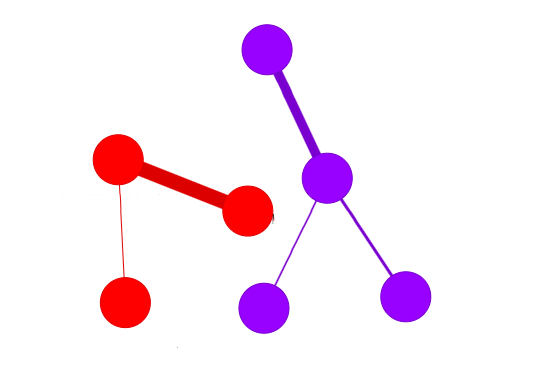
\includegraphics[width=\linewidth]{Minor Thesis/figures/graphs/sa/E.png}
% 		\caption{max(index)-4}
% 	\end{subfigure}
% 	\hfill
% 	\begin{subfigure}[b]{0.13\linewidth}
% 		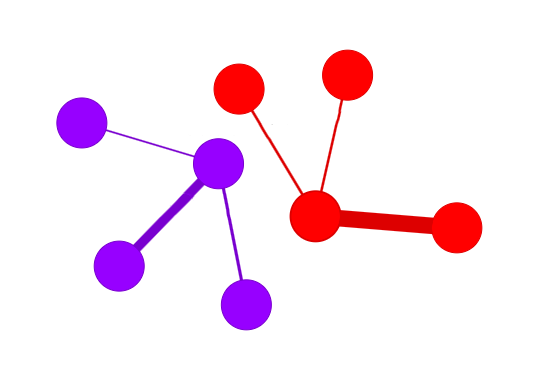
\includegraphics[width=\linewidth]{Minor Thesis/figures/graphs/sa/F.png}
% 		\caption{max(index)-5}
% 	\end{subfigure}
% 	\hfill
% 	\begin{subfigure}[b]{0.13\linewidth}
% 		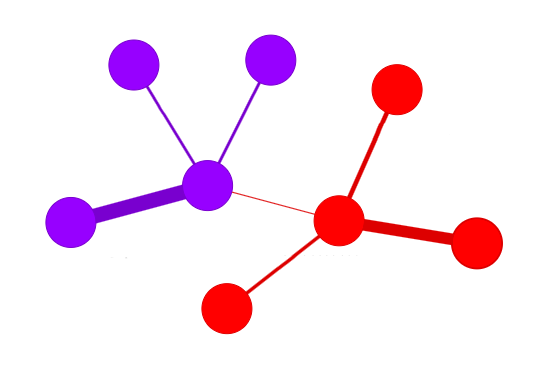
\includegraphics[width=\linewidth]{Minor Thesis/figures/graphs/sa/G.png}
% 		\caption{max(index)-6}
% 	\end{subfigure}
% 	\caption{Graph building evolution. Normalised results using chance weights (success/overall). We indicate values and position as: for (value, index) $\in$ Ascending Ordered Weights, i.e. the highest index contains the highest weight.}
% 	\label{fig:graph-evo-sa}
% \end{figure}
% \FloatBarrier

\subsection{Gain/Loss summaries}
Accuracy may vary along the swapping method, hence can also derive an overview of the general tendency as shown in Figure \ref{fig:gainloss}. The difference score is calculated by subtracting the new accuracy (using the new swapped set) to the old one (original set). If the result is positive, we tag it as \emph{gain}, and otherwise as \emph{loss}. If the scores are exactly the same, we use \emph{equal}.

% Gain/Loss
\begin{figure}[!hptb]
	\centering
% 	\captionsetup{justification=centering}
	\begin{subfigure}[b]{0.45\linewidth}
		\includegraphics[width=\linewidth]{Minor Thesis/figures/gain_loss/swap_Ensemble1000_RCN5333300.png}
		\caption{1000 samples (RCN) 5 Inf, 3 Red, 3 Copy, 3 Cosine, 3 Noise}
	\end{subfigure}
	\hfill
	\begin{subfigure}[b]{0.45\linewidth}
		\includegraphics[width=\linewidth]{Minor Thesis/figures/gain_loss/swap_Ensemble1000_RN5053200.png}
		\caption{1000 samples (RN) 5 Inf, 0 Copy, 5 Red., 3 Cosine, 2 Noise}
	\end{subfigure}
	\caption{Gain/Loss summary on synthetic data. Full lines on each side indicate the maximum value for each group (Gain or Loss). Dashed lines compute the median of the group. The middle line tags the 0 value for reference purposes.}
	\label{fig:gainloss}
\end{figure}
\FloatBarrier

\newpage
\subsection{Swap Score moving threshold}
% 6 Chords
\begin{figure}[!ht]
	\centering
	\begin{subfigure}[b]{0.3\linewidth}
		\includegraphics[width=\linewidth]{figures/chords/chord_swap_Ensemble1000_RCN5333300_095.png}
		\caption{threshold = 0.95}
	\end{subfigure}
	\hfill
	\begin{subfigure}[b]{0.3\linewidth}
		\includegraphics[width=\linewidth]{figures/chords/chord_swap_Ensemble1000_RCN5333300_096.png}
		\caption{threshold = 0.96}
	\end{subfigure}
	\hfill
	\begin{subfigure}[b]{0.3\linewidth}
		\includegraphics[width=\linewidth]{figures/chords/chord_swap_Ensemble1000_RCN5333300_097.png}
		\caption{threshold = 0.97}
	\end{subfigure}
	
	\begin{subfigure}[b]{0.3\linewidth}
		\includegraphics[width=\linewidth]{figures/chords/chord_swap_Ensemble1000_RCN5333300_098.png}
		\caption{threshold = 0.98}
	\end{subfigure}
	\hfill
	\begin{subfigure}[b]{0.3\linewidth}
		\includegraphics[width=\linewidth]{figures/chords/chord_swap_Ensemble1000_RCN5333300_099.png}
		\caption{threshold = 0.99}
	\end{subfigure}
	\hfill
	\begin{subfigure}[b]{0.3\linewidth}
		\includegraphics[width=\linewidth]{figures/chords/chord_swap_Ensemble1000_RCN53333001.png}
		\caption{threshold = 1}
	\end{subfigure}
	\caption{Available relations when increasing the \emph{Swap Score} threshold. Edge thickness indicates strength of relation which is later converted to Rivalry Score. Threshold strictness has a trade-off between accuracy when using high values and completeness when using lower values.}
	\label{fig:six-chords}
\end{figure}
\FloatBarrier

\newpage
\subsection{Extra Histograms}
\label{section:suppl:extra-hist}

% QLOI
\begin{figure}[!htb]
	\centering
	\begin{subfigure}[b]{0.50\linewidth}
		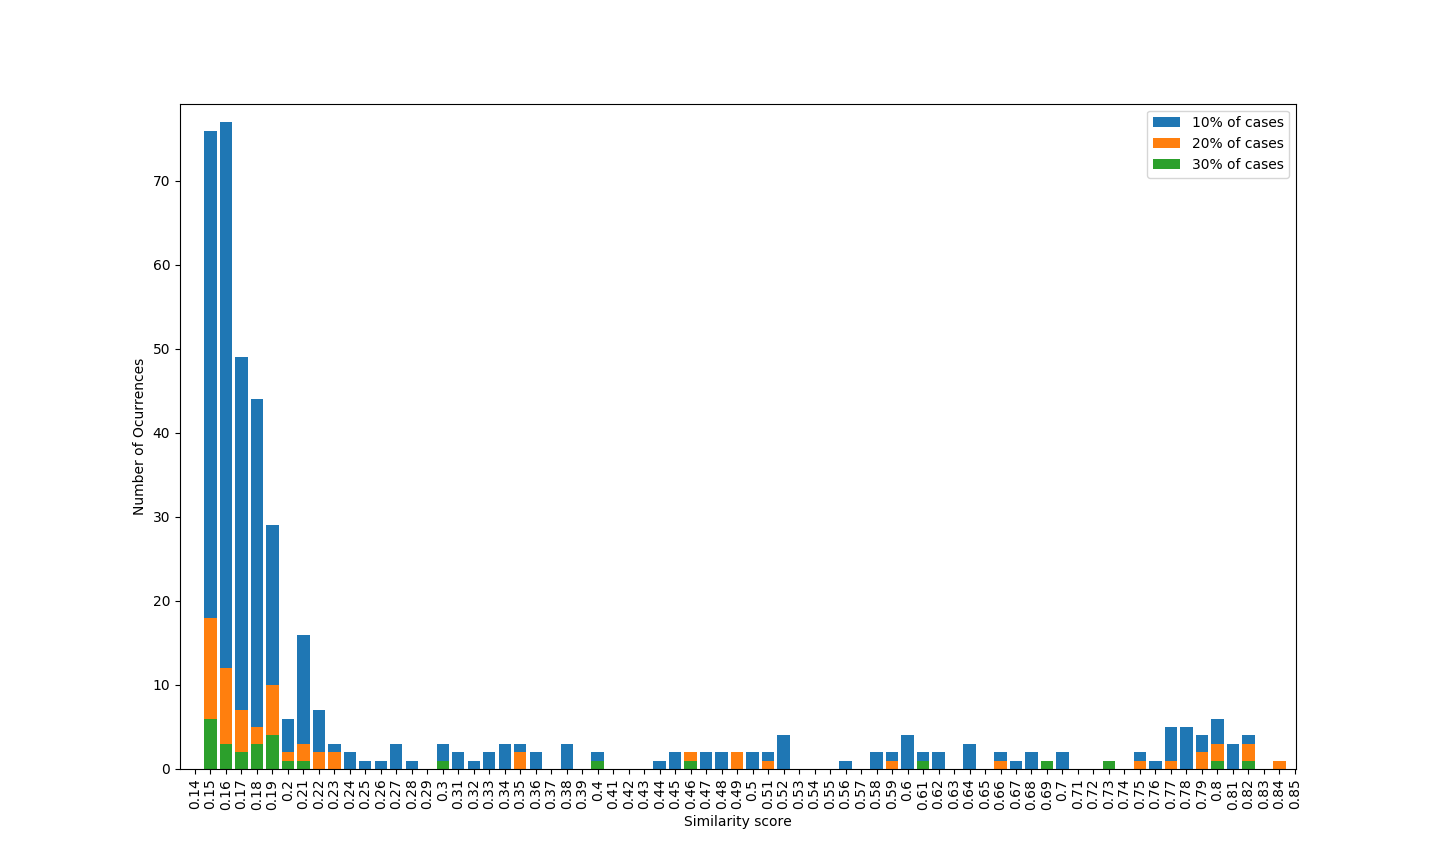
\includegraphics[width=\linewidth]{Minor Thesis/figures/graphs/hist/Hist95.png}
		\caption{Correlation distribution at Swap Score = 0.95}
	\end{subfigure}
	\hfill
	\begin{subfigure}[b]{0.50\linewidth}
		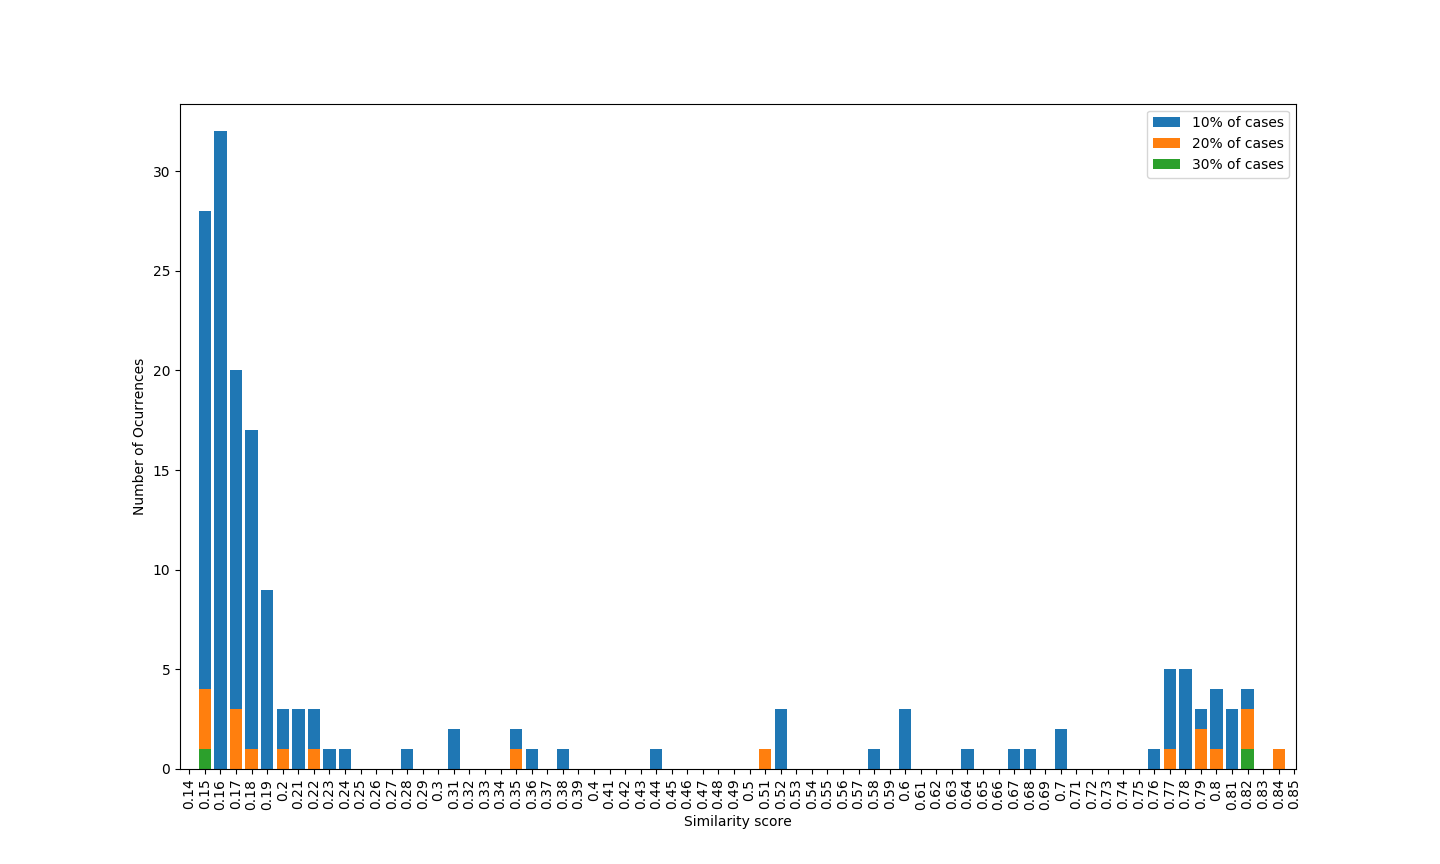
\includegraphics[width=\linewidth]{Minor Thesis/figures/graphs/hist/Hist975.png}
		\caption{Correlation distribution at Swap Score = 0.975}
	\end{subfigure}
	\hfill
	\begin{subfigure}[b]{0.50\linewidth}
		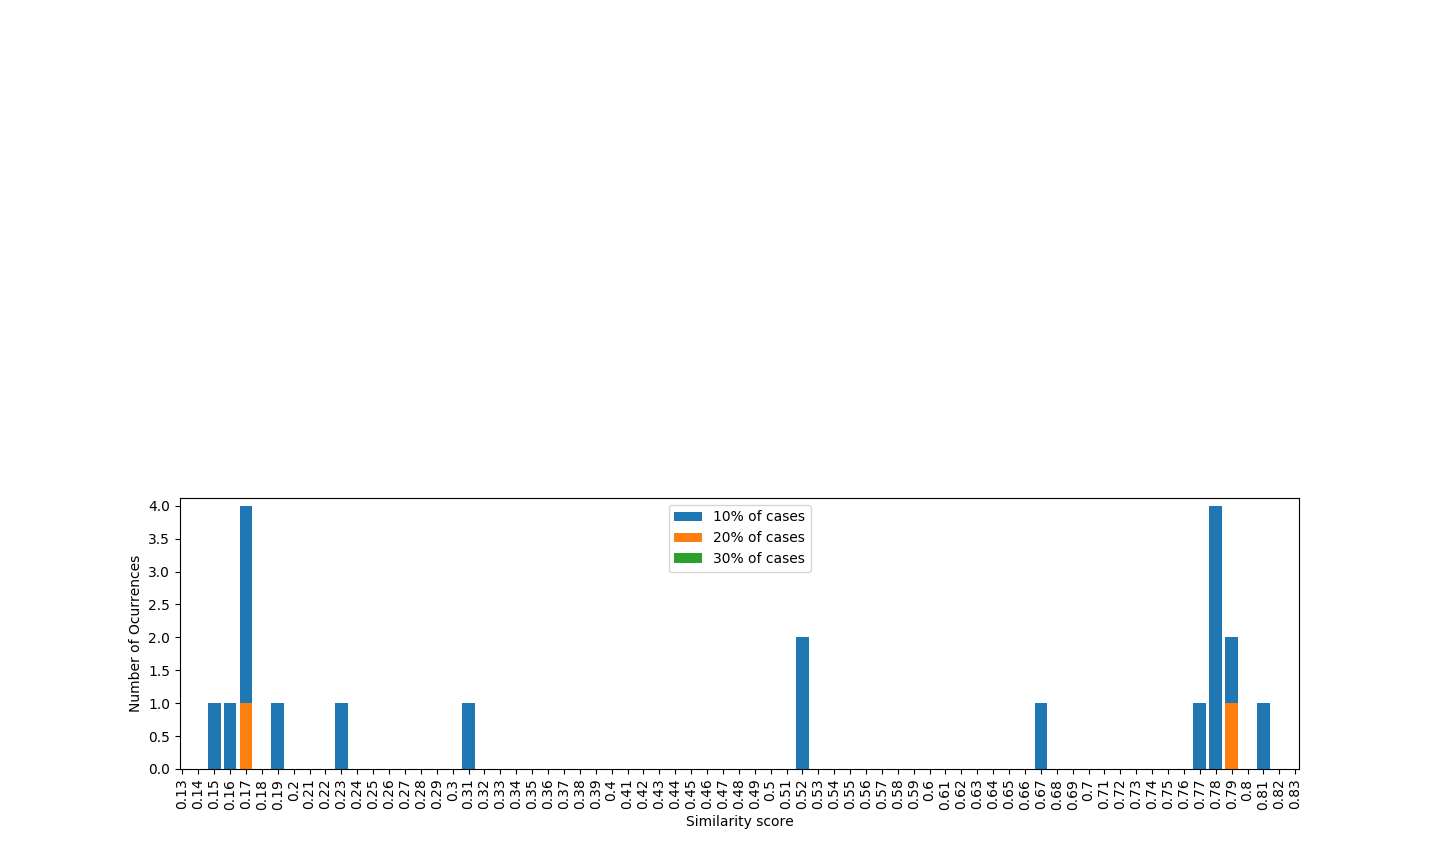
\includegraphics[width=\linewidth]{Minor Thesis/figures/graphs/hist/Hist1.png}
		\caption{Correlation distribution at Swap Score = 1}
	\end{subfigure}	
	\caption{Correlation scores of remaining nodes at different Rivalry Scores.}
	\label{fig:triade-hist}
\end{figure}

% zeroes-count
\begin{figure}[!ht]
    \centering
    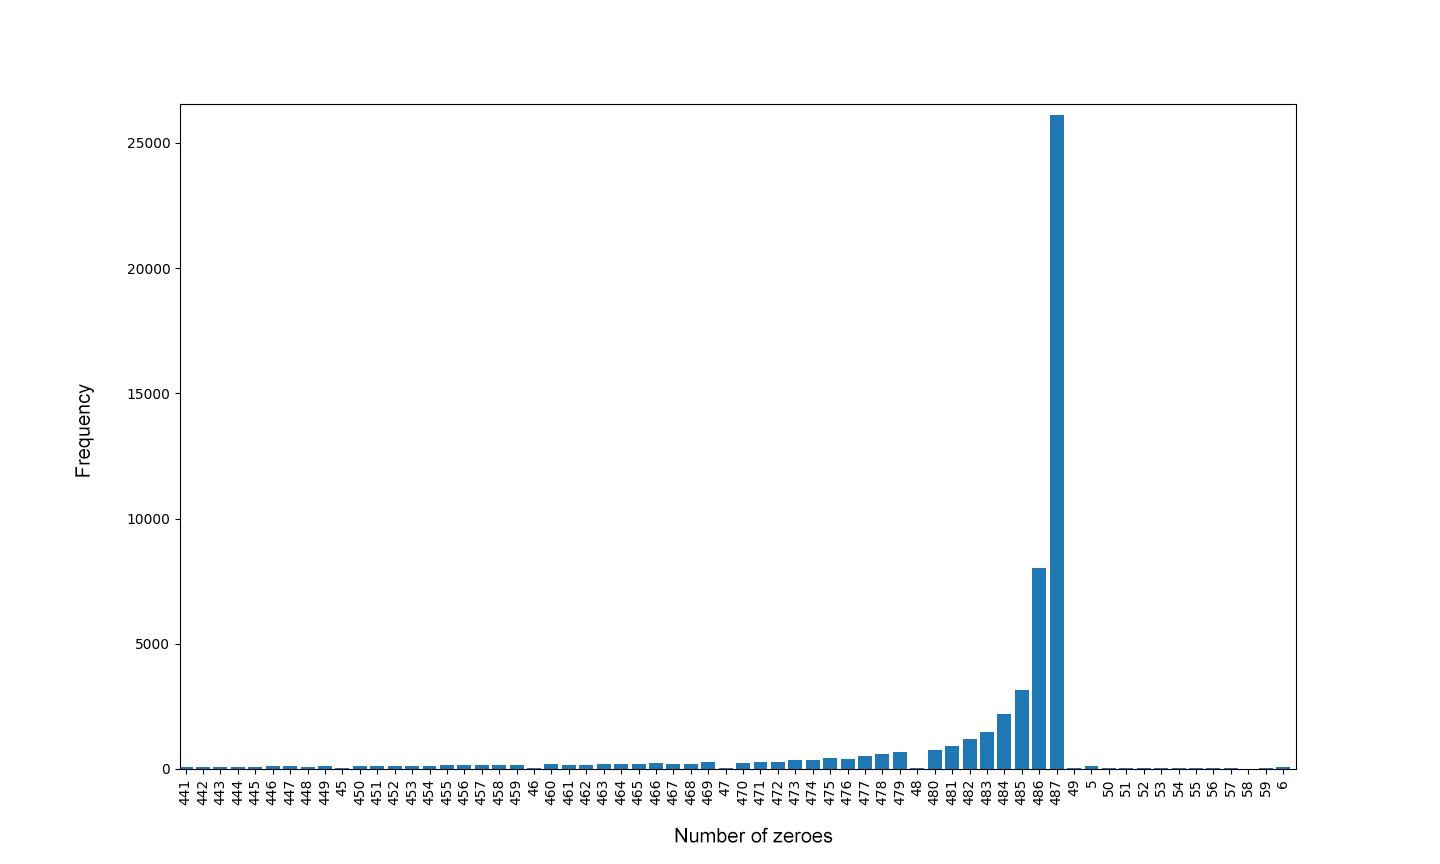
\includegraphics[width=0.75\linewidth]{Minor Thesis/figures/histo/Counter.png}
    \caption{Exploration of values within features. The histogram displays the frequency of variables containing a set number of 0's. Values near 488 are considered to be quasi-constant. The same exploration has been performed to count the number of 1's and 2's (data not shown).}
    \label{fig:counter}
\end{figure}